\section{Experiments}
In this section, we first introduce the experimental setup and the
previous state-of-the-art systems as comparison to 
our own model known as Feature-Enriched-Net.
We then show the implementation details and the evaluation results before
giving some discussion on the results.

\subsection{Training and Testing Data}

We randomly select 500,000 product titles as our training data, 
and another 50,000 for testing.
Each product title $X$ is annotated with a sequence of binary label $Y$,
i.e., each word $x_i$ is labeled with $1$ (included in short title) 
or $0$ (not included in short title). Readers may refer to \secref{sec:data} 
for the details about how we collect the product titles
and their corresponding short titles.

%We augmented each title sentence with the semantic information.
%We extract Term Frequency (TF), Inverse Term Frequency (IDF) and the TF-IDF score for each word in title sentence.
%Besides, we label each word with a tag using an E-commerce Named Entity Recognizer. \xusheng{Should we say it's an inside NER tool from Alibaba?}
%These tags represent the descriptive properties for the product.
%

%To evaluate the accuracy of model inferring with different length of char limit,
%we then split the test data into two parts. 
%In one all the ground-truth short titles are less than 10-chars length (\textbf{10-chars} for short),
%and in another are less than 15-chars (\textbf{15-chars} for short) length.

\subsection{Baseline Systems}
Since there are no previous work that directly solves the short title 
extraction for E-commerce product, we select our baselines from 
three categories. The first one is traditional methods. 
We choose a keyword extraction framework known as 
TextRank \cite{mihalcea2004textrank}.  It first infers an importance 
score for each word within the long title by an algorithm similar to PageRank, 
then decides whether each word should or should not be kept in the short title 
according to the scores.
%We refer to this baseline as TextRank in the rest of the paper.

The second category is standard sequence labeling systems. 
We choose the system mentioned by 
Huang et al.\shortcite{huang2015bidirectional},
in which a muti-layer BiLSTM is used.
Compared to our system, it does not exploit the attention mechanism and 
any side feature information.
We substitute the Conditional Random Field (CRF) layer with 
Logistic Regression to make it compatible with our binary labeling problem.
We call this system BiLSTM-Net.

The last category of methods is attention-based frameworks, 
which use encoder-decoder architecture with attention mechanism.
We choose Pointer Network \cite{vinyals2015pointer} as a comparison and 
call it Pointer-Net.
During decoding, it looks at the whole sentence, calculating the attentional 
distribution and then makes decisions based on the attentional probabilities.
 
%To evaluate the accuracy of different Char-limit Constrained Inference (refer to \secref{sec:infer}) methods,
%we compare our Dynamic Programming algorithm with the simply Greedy implementation as baseline method.
%The Greedy method will select the largest predicted likelihood of term one by one
%until the total length of short title satisfies the constraint.

\subsection{Implementation Details}
We pre-train word embeddings used in our model 
on the whole product titles data plus an extra corpus called 
``E-commerce Product Recommended Reason'',
which is written by online merchants and is also extracted from YouHaoHuo
(\secref{sec:data}).
%\KZ{Where is this data? URL? The name sounds strange..}
%\xusheng{Already explained in Data section, I think it's ok here}
We use the Word2vec \cite{mikolov2013efficient,mikolov2013distributed} 
CBOW model with context window size $5$, negative sampling size $5$, 
iteration steps $5$ and hierarchical softmax $1$. 
The size of pre-trained word embeddings is set to $200$. 
For Out-Of-Vocabulary (OOV) words, embeddings are initialized as zero.
All embeddings are updated during training. 

For recurrent neural network component in our system, 
we used a two-layers LSTM network with unit size $512$.
All product titles are padded to a maximum sentence length of $15$.

We perform a mini-batch cross-entropy loss training with a batch size 
of $128$ sentences for $10$ training epochs.  We use Adam optimizer, 
and the learning rate is initialized with $0.01$.
%Our system is implemented using the popular deep learning framework TensorFlow \cite{abadi2016tensorflow}.

%\section{Results and Discussion}
%In this section, we report experimental results 
%of different systems on product short title extraction.
%The evaluation includs offline comparison and online A/B test. 

\subsection{Offline Evaluation}
\label{sec:eval_offline}
To evaluate the quality of automatically extracted short titles,
we used ROUGE \cite{lin2003automatic} to 
compare model generated
short titles to manually-written short titles.
In this paper, we only report ROUGE-1, mainly because 
linguistic fluency and word order are not of concern in this task.
Unlike previous works in which ROUGE is a recall-oriented metric,
we jointly consider precision, recall and F1 score,
since recall only presents the ratio of 
the number of extracted words included in ground-truth short title
over the total number of words in original long title.
However, due to the limited display space on mobile phones, 
the number of words (or characters) of extracted short title itself 
should be constrained as well.
Thus, precision is also measured in our experiments.
And $ROUGE\textendash1_{F1}$ is considered a comprehensive 
evaluation metric:
\begin{eqnarray*}
& ROUGE\textendash1_{P}=\frac{|S\cap S_{human}|}{|S|},\\
& ROUGE\textendash1_{R}=\frac{|S\cap S_{human}|}{|S_{human}|},\\
& ROUGE\textendash1_{F1}=\frac{2\cdot ROUGE\textendash1_{P}\cdot ROUGE\textendash1_{R}}{ROUGE\textendash1_{P}+ROUGE\textendash1_{R}}.
\end{eqnarray*}
Where $S_{human}$ is the manually written short title, 
and $|S\cap S_{human}|$ is the number of overlapping words appearing 
in short titles generated by model and humans.

Final results on the test set are shown in \tabref{tab:eval1}.
We can find that our method (Feature-Enriched-Net) outperforms the baselines 
on both precision and recall.
Our method achieves the best $0.725$ F1 score, which improves by a relative gain of 4.5\%.
Pointer-Net would achieve higher precision score 
for its attentive ability to the whole sentence and select the most important words.
Our method considers long-short memories, attention mechanism
and other abundant semantic features.
That is to say, our model has the ability to
extract the most essential words from original long titles
and make the short titles more accurate and comprehensive.

We also tune the threshold $\tau$ used in BiLSTM-Net and our Feature-Enriched-Net.
This threshold indicates how large the predicted likelihood should be
so that a word will be included in the final short title.
We reported the results in \figref{fig:eval},
in which we set $\tau$ as $0.3$, $0.4$ and $0.5$.
From the figures, we can conclude that our model stably performs better than
the other.

\begin{table}[htbp]
\centering
\scriptsize
\caption{
	Final results on the test set.
	We report ROUGE-1 Precision, Recall and corresponding F1.
	We use the tuned threshold $\tau=0.4$ (see \figref{fig:eval}) for BiLSTM-Net and Feature-Enriched-Net.
	Best ROUGE score in each column is highlighted in boldface.
}
\label{tab:eval1}
\begin{tabular}{c|ccc}
	\toprule
	Models & $R\textendash1_{P}$ & $R\textendash1_{R}$ & $R\textendash1_{F1}$ \\
	\midrule
	TextRank & 0.430 & 0.219 & 0.290 \\
	BiLSTM-Net & 0.637 & 0.751 & 0.689 \\
	Pointer-Net & 0.648  & 0.746 & 0.694 \\
	Feature-Enriched-Net & \textbf{0.675} & \textbf{0.783} & \textbf{0.725} \\
	\bottomrule
\end{tabular}
\vspace{-10pt}
\end{table}

\begin{figure}[th]
	\centering
	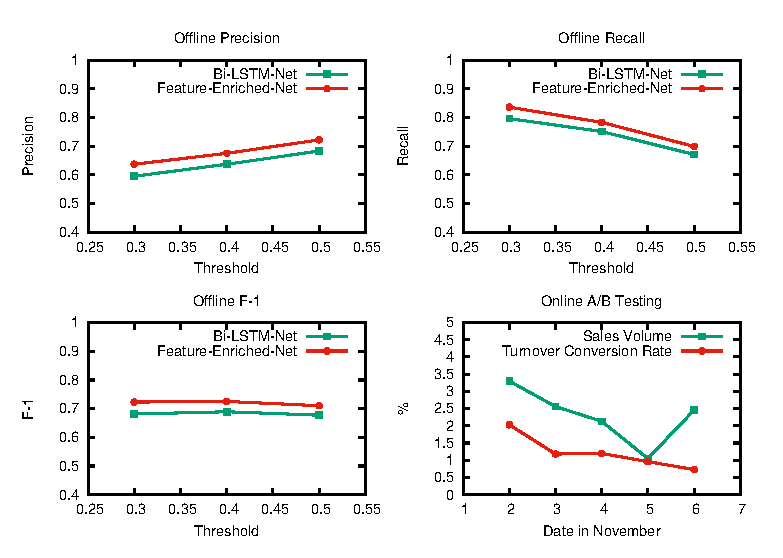
\epsfig{file=fig/exp.eps, angle=0, width=1\columnwidth}
	\caption{Offline results of Bi-LSTM-Net and Feature-Enriched-Net under different thresholds;
	Online A/B Testing of sales volume and 
	Turnover Conversion Rate}
	\label{fig:eval}
%	\vspace{-10pt}
\end{figure}



\subsection{Online A/B Testing}
\label{sec:eval_online}
This subsection presents the results of online evaluation in the search result page scenario
of an E-commerce mobile app with a standard A/B testing configuration.
Due to the limited display space on mobile phones,
only a fixed number of chars (12 characters in this app) 
can be shown out and excessive part will be cut off.
%\KZ{The rest of this para sounds like a method and may be moved to the approach
%sec?}
%\xusheng{I think this part is better put here}
Therefore, unlike previously mentioned inference approach (with threshold $\tau$ in \secref{sec:inference}),
we regard it as classic Knapsack Problem.
Each word $x_i$ in the product title is an item with weight $len(x_i)$ and value $score_i$,
where $len(x_i)$ represents the char length of word $x_i$
and $score_i$ represents the predicted likelihood of word by our model.
The maximum weight capacity of our knapsack is $m$. 
Then the target is:
$$
max \sum_{i=1}^{n} score_i z_i 
$$
$$
s.t. \sum_{i=1}^{n} len(x_i)z_i \le m, z_i \in \{0, 1\}, 
$$
where $z_i=1$ means $x_i$ should be reserved in the short title.
Similar to the standard solution to 0-1 Knapsack Problem,
we use a Dynamic Programming (DP) algorithm. %~\cite{silvano1990knapsack}.

In our online A/B testing evaluation,
3\% of the users were randomly selected as testing group (about 3.4 million user views (UV)),
in which we substituted the original cut-off long title displayed to users
with extracted short titles by our model with DP inference.
We claim that after showing the short titles with most important keywords,
%on search result page, 
users have much better idea what the product is about on the 
``search result'' page and thus find the product they want more easily.
During the popular Double 11 shopping season, 
we deployed A/B testing for 5 days (from 2017-11-02 to 2017-11-06) 
and achieved on average \textbf{2.31\%} and \textbf{1.22\%} improvements of 
sales volume and turnover conversion rate (see \figref{fig:eval} for each day).
This clearly shows that better short product titles are more user-friendly
and hence improve the sales substantially.
%\yu{IPV decreases because users clearly know the products by short title and will not click to check them,	but turnover conversion rate increases more. So that totally sales volume is improved.}

\begin{table*}[ht]
	\scriptsize
	\centering
	\caption{A real experimental case with 12-chars length limit.
		%for original long title, human annotated short title, BiLSTM-Net and Feature-Enriched-Net generated short title with DP inference (12 characters length limit). 
		Pointer-Net is not included since encoder-decoder architecture can't directly adapt to character length limit}
	\label{tab:case_study}
	\begin{tabular}{c|c}
		\toprule
		\multirow{2}{*}{ORIGINAL} & xunruo 熏 若 双生 设计师 品牌 泡泡 系列 一 字领 掉 袖 连衣裙 预订 款  \\
		& (Bookable XunRuo twin designer brand bubble series dress with boat neckline and off sleeves.) \\ 
		\midrule
		\multirow{2}{*}{HUMAN} & 一字领 掉 袖 连衣裙 \\
		& (Dress with boat neckline and off sleeves.) \\
		\midrule
		\multirow{2}{*}{Feature-Enriched-Net} & 泡泡 系列 一字领 掉 袖 连衣裙 \\
		& (Bubble series dress with boat neckline and off sleeves.) \\
		\midrule
		\multirow{2}{*}{BiLSTM-Net} & 熏 若 品牌 掉 袖 连衣裙 预订\\
		& (Bookable XunRuo brand dress with off sleeves.) \\
		%\midrule
		%Pointer-Net & --- \\
		\bottomrule
	\end{tabular}
\end{table*}


\subsection{Discussion}
In \tabref{tab:case_study}, we show a real case of original long title, 
along with short title annotated by human beings, 
predicted by BiLSTM-Net and Feature-Enriched-Net respectively.
From the human annotated short title,
we find that a proper short title should contain 
the most important elements of the product,
such as category (``dress'') and description of properties (``boat neckline and off sleeves'').
While some other elements such as 
brand terms (``XunRuo twin designer brand'')
or service terms (``open for reservation'') 
should not be kept in the short title.
Our Feature-Enriched Net has the ability to generate
a satisfying short title,
while baseline model tends to miss some essential information.

However, there is still room for improvement.
Word terms with similar meaning may co-occur
in the short title generated by our model,
when they happen to be important words such as a category.
For example, 
``皮衣''and``皮夹克'' both mean ``jacket'' in a long title,
and the model tends to keep both of them.
However, only one of them is enough and
the space saved can be used to display other useful information to customers.
We will explore intra-attention \cite{paulus2017deep} as an extra feature in our future work.

%\yu{Add negative example.}
%Original long title is ``欧美 大牌 定制 蛇纹 印花 时尚 机车 皮衣 女 真皮 皮夹克 绵羊皮 外套 短款'',ground truth short title is ``蛇纹 印花 机车 皮衣''
%and predicted short title is ``蛇纹 印花 机车 皮衣 皮夹克''.


%\begin{CJK}{UTF8}{gbsn}
%\begin{table*}
%	\centering
%	\label{tab:demo}
%	\begin{tabular}{c|c|c}
%		\toprule
%		Product Title & Ground-truth Short Title &  12-Char Limit Constrained Inference  \\
%		\midrule
%		taijizen 太极禅 &
%		\multirow{4}{*}{中国风 复古 简约 女装 棉质 百搭 马甲}
%		&  \multirow{4}{*}{\textbf{中国风} \textbf{复古} \textbf{棉质} \textbf{百搭} \textbf{马甲}} \\
%		新款 时尚 中国风 & & \\
%		复古 简约 女装 & & \\
%		棉质 百搭 马甲 & & \\
%		\midrule
%		欧美 大牌 定制 蛇纹 &
%		\multirow{4}{*}{蛇纹 印花 机车 皮衣} & \multirow{4}{*}{\textbf{蛇纹} \textbf{印花} \textbf{机车} \textbf{皮衣} 皮夹克} \\
%		印花 时尚 机车 皮衣 & & \\
%		女 真皮 皮夹克 & & \\
%		绵羊皮 外套 短款 & & \\
%		\midrule
%		正品 代购 秋冬 
%		& \multirow{4}{*}{女 宽松 加绒 运动 卫裤} & 	\multirow{4}{*}{\textbf{宽松} \textbf{加绒} 哈伦裤 \textbf{运动} \textbf{卫裤}} \\
%		新款 女 宽松 加绒 & & \\
%		哈伦裤 保暖 休闲 & & \\
%		运动 卫裤 现货 & & \\
%		\midrule
%		准时 开 抢 
%		& \multirow{4}{*}{乐瓣 春装 新款 女 圆领 套头 宽松 卫衣} & \multirow{4}{*}{\textbf{乐瓣} \textbf{女} \textbf{圆领} \textbf{套头} \textbf{宽松} \textbf{卫衣}} \\ 
%		乐瓣 春装 新款 & & \\
%		女 圆领 套头 & & \\
%		宽 松 卫衣 & & \\
%		\midrule
%		xunruo 熏 若 
%		& \multirow{5}{*}{一字领 掉 袖 连衣裙} & \multirow{5}{*}{泡泡 系列 \textbf{一字领} \textbf{掉} \textbf{袖} \textbf{连衣裙}} \\
%		双生 设计师 品牌 & & \\
%		泡泡 系列 一 字领 & & \\
%		掉 袖 连衣裙 & & \\
%		预订 款 & & \\
%		\bottomrule
%	\end{tabular}
%	\caption{}
%\end{table*}
%\end{CJK}

